\documentclass[tikz,border=10pt]{standalone}
\usepackage{fontspec}
\usepackage{xeCJK}
\setmainfont{Times New Roman}
\setCJKmainfont{Hiragino Sans GB}
\setCJKsansfont{Microsoft YaHei}
\setCJKmonofont{STSong}
\usepackage{tikz}
\usetikzlibrary{arrows.meta,positioning}

\tikzset{
  block/.style={draw=blue!70!black, line width=1.2pt, minimum width=2.0cm, minimum height=0.95cm, align=center, fill=none},
  sum/.style={circle, draw=green!50!black, line width=1.2pt, minimum size=7mm, inner sep=0pt},
  signal/.style={-{Stealth[length=3mm]}, line width=1.2pt, draw=black!70}
}

\begin{document}
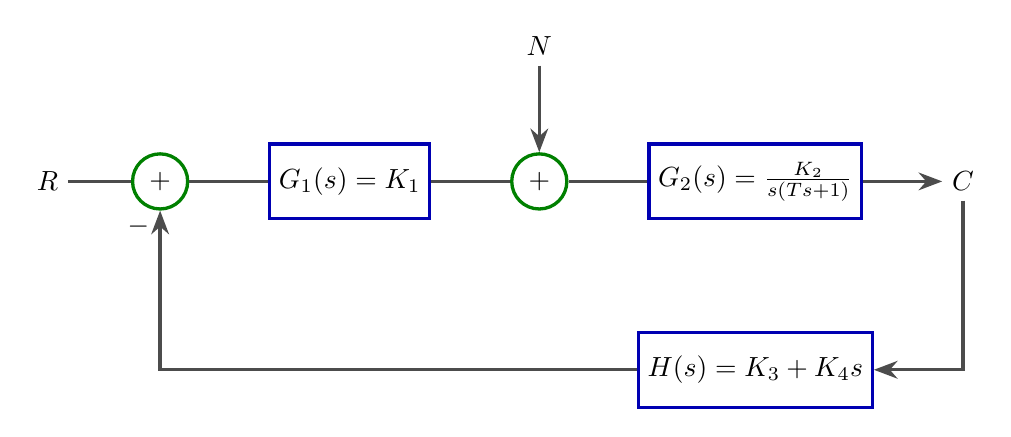
\begin{tikzpicture}[node distance=0.9cm and 0.9cm]
  \node (r) {$R$};
  \node[sum, right=0.8cm of r] (s1) {$+$};
  \node[block, right=1.0cm of s1] (g1) {$G_1(s)=K_1$};
  \node[sum, right=1.0cm of g1] (s2) {$+$};
  \node[block, right=1.0cm of s2] (g2) {$G_2(s)=\frac{K_2}{s(Ts+1)}$};
  \node[right=1.0cm of g2] (c) {$C$};
  \node[above=1.1cm of s2] (n) {$N$};
  \node[block, below=1.4cm of g2] (h) {$H(s)=K_3+K_4 s$};

  \draw[signal] (r) -- (s1) -- (g1) -- (s2) -- (g2) -- (c);
  \draw[signal] (n) -- (s2);
  \draw[signal] (c) |- (h);
  \draw[signal] (h) -| node[pos=0.95,left] {$-$} (s1.south);
\end{tikzpicture}
\end{document}
